\documentclass[10pt,conference]{IEEEtran}
% \documentclass[10pt]{article}
\IEEEoverridecommandlockouts
\usepackage{cite}
\usepackage{amsmath,amssymb,amsfonts}
\usepackage{algorithmic}
\usepackage{graphicx}
\usepackage{textcomp}
\usepackage{xcolor}
\usepackage[backref]{hyperref}
\usepackage{booktabs}
\def\BibTeX{{\rm B\kern-.05em{\sc i\kern-.025em b}\kern-.08em
    T\kern-.1667em\lower.7ex\hbox{E}\kern-.125emX}}

\begin{document}

\title{\textbf{Coursework 3}: System-level Performance\\
Evaluation of 5G New Radio MIMO Downlink
}

\author{\IEEEauthorblockN{Zhaolin Wang}}

\maketitle

\section{Task 1: System Model}
This coursework aims at investigating the performance of LTE 4G Single-User
MIMO. The base station (BS) servers $K$ user equipments (UEs) in the center
cell. The transmission is subject to the interference from the neighboring BS.
We assume that there are $n_t$ antennas at the BS and $n_r$ antennas at the 
UEs.

In the center cell, the BS schedules one UE at a time, and the Spatial Multiplexing
with quantized precoding is exploited. The signal transmitted from BS $i$
to user $q$ at time $k$ is given as
\begin{equation}
    {\bf{x}}_{q,i} = \underbrace{{\bf{W}}_{q,i} {\bf{S}}_{q,i}^{1/2}}_{{\bf{P}}_{q,i}} {\bf{c}}_{q,i} \label{eq1}
\end{equation}
where the ${\bf{W}}_{q,i} \in {\mathbb{C}}^{n_t \times r}$ is the precoder
selected from the codebook, ${\bf{S}}_{q,i} \in {\mathbb{C}}^{r \times r}$ 
is a diagonal matrix controlling the power allocation, and ${\bf{c}}_{q,i} \in {\mathbb{C}}^{r \times 1}$
are the transmitted symbols. The $r$ is determined by the Rank Indicator (RI)
fed back from the user $q$, and there must be $r \leq \min\{n_r,n_t\}$. 
The observation at user $q$ is given as 
\begin{equation}
    {\bf{y}}_{q} = \Lambda_{q,i}^{-1/2} {\bf{H}}_{q,i} {\bf{x}}_{q,i} + \underbrace{\sum_{j \neq i} \Lambda_{q,j}^{-1/2} {\bf{H}}_{q,j} {\bf{x}}_{q,j}}_{\text{inter-cell interference}} + {\bf{n}}_{q} \label{eq2}
\end{equation}
where the $\Lambda_{q,i}$ is the large scale fading determined by the path loss
and the showing, ${\bf{H}}_{q,i} \in \mathbb{C}^{n_r \times n_t}$ is the 
Rayleigh fading matrix from BS $i$ to user $q$, and ${\bf{n}}_{q} \in \mathbb{C}^{n_r \times 1}$ 
is the noise vector whose entries are the complex Gaussian distribution 
$\mathcal{CN} (0,\sigma_n^2)$. 

\subsection{MMSE Receiver}
Define the interference and noise as
\begin{equation}
    \begin{split}
        \tilde{{\bf{n}}}_{q} & = \sum_{j \neq i} \Lambda_{q,j}^{-1/2} {\bf{H}}_{q,j} {\bf{x}}_{q,j} + {\bf{n}}_{q} \\
        & = \sum_{j \neq i} \Lambda_{q,j}^{-1/2} {\bf{H}}_{q,j} {\bf{P}}_{q,j} {\bf{c}}_{q,j} + {\bf{n}}_{q} \label{eq3}
    \end{split}
\end{equation}
Then the covariance matrix of noise plus interference is denoted by
\begin{equation}
    \begin{split}
        {\bf{R}}_{\tilde{{\bf{n}}}_{q}} & = \mathbb{E}[\tilde{{\bf{n}}}_{q} \tilde{{\bf{n}}}_{q}^H]\\
        & = \sum_{j \neq i} \Lambda_{q,j}^{-1} {\bf{H}}_{q,j} {\bf{P}}_{q,j} {\bf{P}}_{q,j}^H {\bf{H}}_{q,j}^H + \sigma_n^2 {\bf{I}}_{n_r \times n_r}\label{eq4}
    \end{split}
\end{equation}
According to \eqref{eq1}\eqref{eq2}\eqref{eq4}, the MMSE combiner is given as
\begin{equation}
    \begin{split}
        {\bf{G}}_q^{\text{MMSE}} & = \arg \min_{{\bf{G}}_q} ||{\bf{G}}_q {\bf{y}}_q - {\bf{c}}_{q,i}||^2\\
        & = \Lambda_{q,j}^{-1/2} {\bf{P}}_{q,i}^H {\bf{H}}_{q,i}^H (\Lambda_{q,j}^{-1} {\bf{H}}_{q,i} {\bf{P}}_{q,i} {\bf{P}}_{q,i}^H {\bf{H}}_{q,i}^H + {\bf{R}}_{\tilde{{\bf{n}}}_{q}})^{-1} \label{eq5}
    \end{split}
\end{equation}

Alternatively, considering the $l$-th stream in the signal, the \eqref{eq2}
can be rewritten as
\begin{equation}
    \begin{split}
        {\bf{y}}_{q} = \Lambda_{q,i}^{-1/2} {\bf{H}}_{q,i} {\bf{p}}_{q,i,l} c_{q,i,l} + \underbrace{\sum_{m \neq l} \Lambda_{q,i}^{-1/2} {\bf{H}}_{q,i} {\bf{p}}_{q,i,m} c_{q,i,m}}_{\text{inter-stream interference}} \\
        + \underbrace{\sum_{j \neq i} \Lambda_{q,j}^{-1/2} {\bf{H}}_{q,j} {\bf{x}}_{q,j}}_{\text{inter-cell interference}} + {\bf{n}}_{q}. \label{eq6}
    \end{split}
\end{equation}
Denote the noise plus interference for stream $l$ at user $q$ by
\begin{equation}
    \tilde{{\bf{n}}}_{q,l} = \sum_{m \neq l} \Lambda_{q,i}^{-1/2} {\bf{H}}_{q,i} {\bf{p}}_{q,i,m} c_{q,i,m} 
        + \sum_{j \neq i} \Lambda_{q,j}^{-1/2} {\bf{H}}_{q,j} {\bf{x}}_{q,j} + {\bf{n}}_{q}.\label{eq7}
\end{equation}
Its covariance matrix is given by
\begin{equation}
    \begin{split}
        {\bf{R}}_{\tilde{{\bf{n}}}_{q,l}} & = \mathbb{E}[\tilde{{\bf{n}}}_{q,l} \tilde{{\bf{n}}}_{q,l}^H]\\
        & = \sum_{m \neq l} \Lambda_{q,i}^{-1} {\bf{H}}_{q,i} {\bf{p}}_{q,i,m} {\bf{p}}_{q,i,m}^H {\bf{H}}_{q,i}^H \\
        & + \sum_{j \neq i} \Lambda_{q,j}^{-1} {\bf{H}}_{q,j} {\bf{P}}_{q,j} {\bf{P}}_{q,j}^H {\bf{H}}_{q,j}^H + \sigma_n^2 {\bf{I}}_{n_r \times n_r}  \label{eq8}  
    \end{split}
\end{equation}
Therefore, the MMSE combiner for stream $l$ is:
\begin{equation}
    {\bf{g}}_{q,l}^{\text{MMSE}} = \Lambda_{q,i}^{-1/2}({\bf{H}}_{q,i} {\bf{p}}_{q,i})^H {\bf{R}}_{\tilde{{\bf{n}}}_{q,l}}^{-1} \label{eq9}
\end{equation}
The output of MMSE at stream $l$ is given as
\begin{equation}
    {\bf{g}}_{q,l}^{\text{MMSE}} {\bf{y}}_q = \Lambda_{q,i}^{-1/2} {\bf{g}}_{q,l}^{\text{MMSE}} {\bf{H}}_{q,i} {\bf{p}}_{q,i,l} c_{q,i,l} + {\bf{g}}_{q,l}^{\text{MMSE}} \tilde{{\bf{n}}}_{q,l} \label{eq10}
\end{equation}
According to \eqref{eq10}, the output SINR of MMSE at stream $l$ is
\begin{equation}
    \begin{split}
        \rho_{q,l} & = \frac{\Lambda_{q,i}^{-1} |{\bf{g}}_{q,l}^{\text{MMSE}} {\bf{H}}_{q,i} {\bf{p}}_{q,i,l}|^2} {{\bf{g}}_{q,l}^{\text{MMSE}} {\bf{R}}_{\tilde{{\bf{n}}}_{q,l}} ({\bf{g}}_{q,l}^{\text{MMSE}})^H}\\
        & = \Lambda_{q,i}^{-1} {\bf{p}}_{q,i,l}^H {\bf{H}}_{q,i}^H {\bf{R}}_{\tilde{{\bf{n}}}_{q,l}}^{-1} {\bf{H}}_{q,i} {\bf{p}}_{q,i,l} \label{eq11}
    \end{split}
\end{equation}
The overall achievable rate for user $q$ is
\begin{equation}
    R_q = \sum_{l=1}^{r} \log_2(1 + \rho_{q,l}) \label{eq12}
\end{equation}

\subsection{Spatial Multiplexing with Quantized Precoding}
The limited amount of feedback at the transmitter is assumed in this coursework.
In this case, the quantized precoding is applied, where the precoder
${\bf{W}}_{q,i}$ is selected from a finite set of precoders. This coursework
concentrates on the scenario where $n_t$=4, therefore the LTE 4Tx codebook is used.

At the user $q$, a Precoding Matrix Indicator (PMI), a Channel Quality indicator,
and a Rank Indicator will be decided by the receiver and transmitted back to 
the BS. The PMI and RI determine which precoder in the codebook will be applied.
In this procedure, the precoder is chosen with rank adaptation and rate maximization.
\begin{equation}
    {\bf{W}}_{q,j}^* = \arg \max_{r} \max_{{\bf{W}} \in \mathcal{W}_r} R_q \label{eq13}
\end{equation}
where $\mathcal{W}_r$ is the codebook defined for rank $r$ ($r \leq \min\{n_r,n_t\}$).

\subsection{Proportional Fair Scheduling}
In the LTE 4G Single-User MIMO, the BS in the center cell schedules one user 
at a time. In order to guarantee the fairness among the user, the proportioanl
fair metric is relied on, where the weighted sum-rate is maximized. At each time
instance $k$, the user $q^*$ is scheduled based on
\begin{equation}
    q^* = \arg\max_q \frac{R_q(k)}{\bar{R}_q(k)} \label{eq14}
\end{equation}
where $R_q(k)$ is the instantaneous achievable rate of user $q$ and $\bar{R}_q(k)$
is the long-term average rate, which is updated as
\begin{equation}
    % \bar{R}_q(k+1) = \begin{cases} (1-1/t_c)\bar{R}_q(k) + 1/t_c R_q(k) &q \text{ scheduled at time } k \\
    %                                (1-1/t_c)\bar{R}_q(k)\end{cases} &q \text{ scheduled at time } k
    \bar{R}_q(k+1)=\begin{cases} (1-1/t_c)\bar{R}_q(k) + 1/t_c R_q(k),& q \text{ scheduled}\\(1-1/t_c)\bar{R}_q(k),& q\text{ not scheduled} \end{cases} \label{eq15}
\end{equation}
where $t_c$ is the scheduling time scale. 

\subsection{MIMO Channel Model}
The uncorrelated flat fading MIMO channel is assumed following the first-order Gauss-Markov
process
\begin{equation}
    \tilde{{\bf{H}}}_{k,q,i} = \epsilon \tilde{{\bf{H}}}_{k-1,q,i} + \sqrt{1-\epsilon^2} \tilde{{\bf{N}}}_{k,q,i} \label{eq16}
\end{equation}
The actual MIMO channel is given as
\begin{equation}
    {\bf{H}}_{k,q,i} = \tilde{{\bf{H}}}_{k,q,i} {\bf{R}}_{t,q,i}^{1/2} \label{eq17}
\end{equation}
where ${\bf{R}}_{k,q,i}$ is the transmit correlation matrix, which is given as
\begin{equation}
    {\bf{R}}_{t,q,i} = \left[  \begin{matrix} 1 & t_{q,i} & t_{q,i}^2 & t_{q,i}^3\\
        t_{q,i}^* & 1 & t_{q,i} & t_{q,i}^2\\
        t_{q,i}^{2*} & t_{q,i}^* & 1 & t_{q,i}\\
        t_{q,i}^{3*} & t_{q,i}^{2*} & t_{q,i}^* & 1\end{matrix}\right] \label{eq18}
\end{equation}
where $t_{q,i}=0, \forall i \neq 0$ and $t_{q,0}=te^{j \phi_q}$ where $t$ is the magnitude
and $\phi_q$ is the phase randomly distributed between $0$ and $2\pi$.

\subsection{User Location}
The UEs are randomly and uniformly dropped at a distance $> 35m$ and $< 250m$ from 
the BS. Figure \ref{fig1} shows one realization of the UE locations for $K=10$.
\begin{figure}
    \centering
    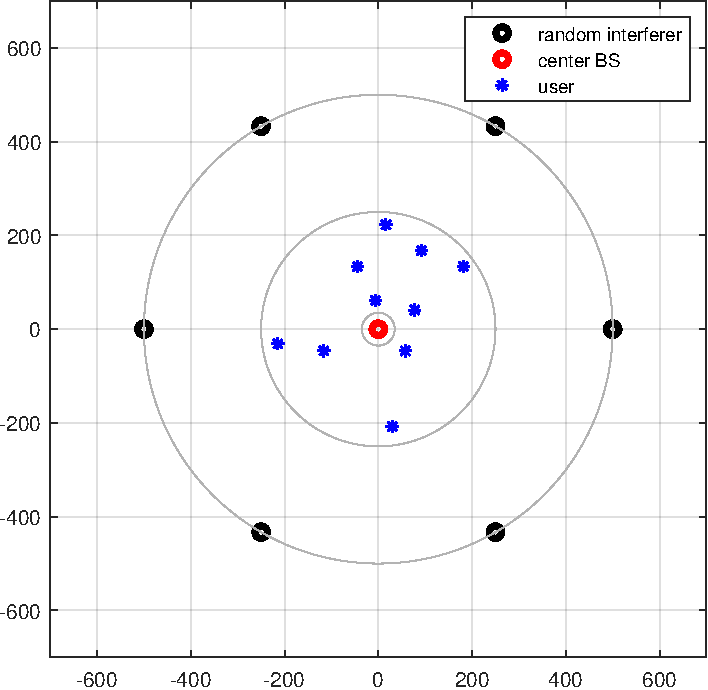
\includegraphics[width=1\linewidth]{Fig1.pdf}
    \caption{Locations of UEs ($K=10$)}
    \label{fig1}
\end{figure}

\section{Task 2: CDF of the long term SINR}
For user $q$ in cell $i$, the long term SINR is given by 
\begin{equation}
    SINR_{LT,q} = \frac{\Lambda{q,i}^{-1} E_{s,i}}{\sigma^2_{n,q} + \sum_{j \neq i} \Lambda_{q,j}^{-1} E_{s,j}} \label{eq19}
\end{equation}
In this task, $10^6$ user locations are randomly generated and 
the long term SINR is calculated according to \eqref{eq19}.

\begin{figure}[htb]
    \centering
    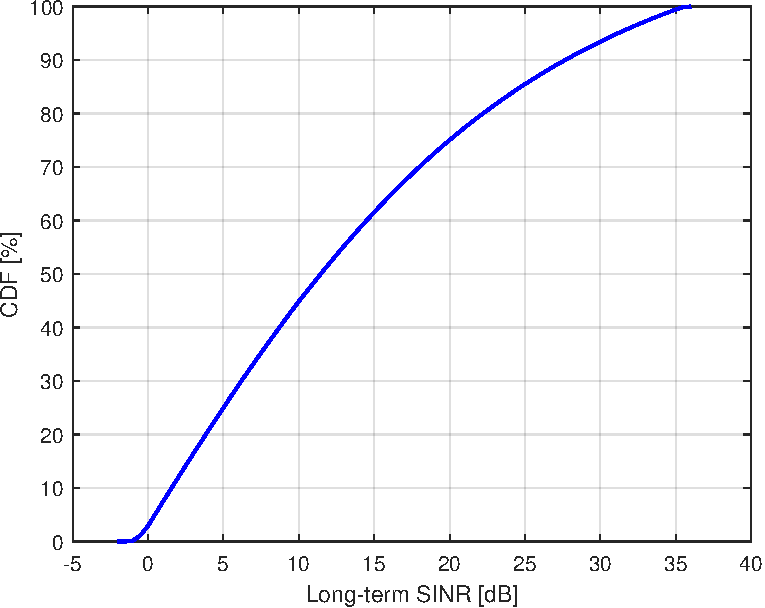
\includegraphics[width=1\linewidth]{Fig2.pdf}
    \caption{CDF of the user long term SINR}
    \label{fig2}
\end{figure}

Figure \ref{fig2} shows the CDF of the long term SINR. It is clear that the 
long term SINR is varying from -1.2dB to 35.6dB.

\section{Task 3: Influence of the number of receive antennas}
For all the following task, the power is uniformly allocated to each streams.
The precoders at the neighbouring BS are randomly selected from the codebook.
The average user rate is calculated over 800 time instances during which the proportional 
fairness scheduling is stable. The CDF is calculated by taking 500 random drops of users.
The parameters of baseline for all the following tasks are 

\begin{table} [htb]
    \caption{Baseline Parameters}
    \centering
    \setlength{\tabcolsep}{8mm}{
        \centering
        \begin{tabular}{ll}% 通过添加 | 来表示是否需要绘制竖线
            \toprule
            Parameter & Value\\\hline

            Receive Antennas $n_r$ & 1\\

            User Number $K$ & 10\\

            Transmit Power $P_t$ & 46dBm\\

            Noise Power $\sigma_n^2$& -174dBm\\

            Spatial Correlation $t$ & 0.5\\

            Time Correlation $\epsilon$ & 0.85\\

            Scheduling Time Scale $t_c$ & 50\\

            \bottomrule
        \end{tabular} \label{table1}
    }
\end{table}

Figure \ref{fig3} shows the CDF of user average rate in the case of 
different receive antennas. It is obvious that the system have better performance
if $n_r=2$. Compared with $n_r=1$, the maximum average user rate is increased by 
0.7 bps/Hz and minimum average user rate in increased by 0.25 bps/Hz.
The reason is that the maximum value of the rank of channel 
matrix is $r=2$, therefore the system is capable of supporting 
2 streams and there is a multiplexing gain. But for $n_r=1$, maximum number of streams
can be supported is 1, and there is no multiplexing gain exploited. Even though there is only
1 stream transmitted for $n_r=2$, there is also diversity gain can be exploited at the 
MMSE receiver, because the MMSE receiver firstly whitens the coloured 
noise (i.e., interference plus noise) and then performs the maximum ratio combining. 
Therefore, the case $n_r=2$ outperforms the case $n_r=1$ in terms of both
multiplexing gain and diversity gain.

% However, the two cases have almost the same lower bound (0.3 bps/Hz) of 
% average user rate. The reason is that the rank of channel matrix for 
% $n_r=2$ is not always 2 because of the spatial correlation. 
% If the rank of channel matrix is 1, the system for $n_r=2$ can also only 
% support one stream although there are two  receive antennas, where the average 
% user rate can reach the same lower bound as that in the case of $n_r=1$.

\begin{figure} [htb]
    \centering
    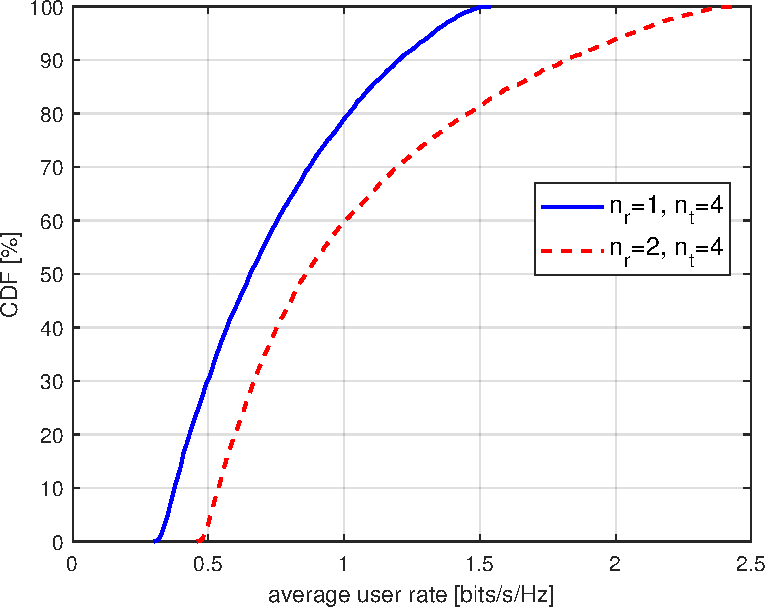
\includegraphics[width=1\linewidth]{Fig3.pdf}
    \caption{CDF of user average rate in the case of different receive antennas}
    \label{fig3}
\end{figure}

\section{Task 4: Influence of the scheduling time scale}

Figure \ref{fig4} shows the CDF of user average rate in the case of 
scheduling time scales. The average user rate is worst when $t_c=1.1$, whose 
minimum value is 0.1 bps/Hz lower than that of $t_c=50$ and maximum value is 0.2 
bps/Hz lower than that of $t_c=50$. There is also increase of average user rate when 
$t_c$ increases from 50 to $10^4$, but it is not very significant.
It is clear that the higher scheduling time scale 
$t_c$ in \eqref{eq15} results in the better performance of average user rate.

\begin{figure} [htb]
    \centering
    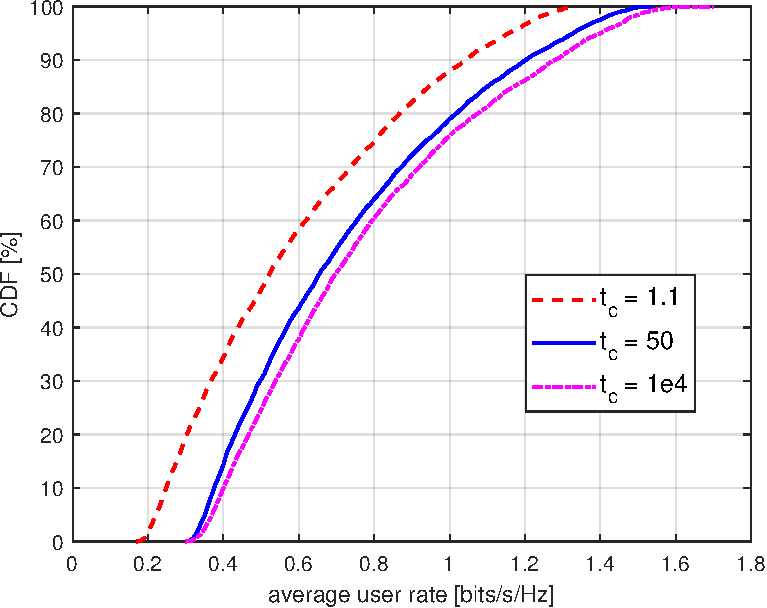
\includegraphics[width=1\linewidth]{Fig4.pdf}
    \caption{CDF of user average rate in the case of different scheduling time scales}
    \label{fig4}
\end{figure}

For the very large $t_c$, the long-term average rate in \eqref{eq15} becomes
\begin{equation}
    \lim_{t_c \rightarrow \infty}\bar{R}_q(k+1) = \begin{cases} \bar{R}_q(k),& q \text{ scheduled}\\\bar{R}_q(k),& q\text{ not scheduled} \end{cases} \label{eq20}
\end{equation}
It means that for the very large $t_c$, the $\bar{R}_q$ only changes very little
at each time instance, and almost keep constant. Therefore, when choosing which 
user is scheduled at each time instance $k$ based on the criterion \eqref{eq14},
the instantaneous rate $R_q(k)$ will dominant the result of selection, i.e.,
the user with the highest instantaneous rate $R_q(k)$ compared with its $\bar{R}_q$ will 
be more likely to be scheduled. There will also be multi-user diversity to 
be exploited. Nevertheless, the drawback of large $t_c$ is the low fairness 
among the user, as the users with weak channel state have very low 
opportunity to be scheduled. 

For the small $t_c$, the long-term rate becomes
\begin{equation}
    \lim_{t_c \rightarrow 1}\bar{R}_q(k+1) = \begin{cases} R_q(k),& q \text{ scheduled}\\0,& q\text{ not scheduled} \end{cases} \label{eq21}
\end{equation}
If the user $q$ is not scheduled at time $k$, the $\bar{R}_q(k+1)$ will directly drop to 
almost zero. In this case, $R_q(l+1) / \bar{R}_q(k+1) \rightarrow \infty$, and the 
scheduler will equally select from the users which are not scheduled at time $k$
based on \eqref{eq14}. Therefore, there is no multi-user diversity gain exploited, 
resulting in the lower performance of average user rate. However, the fairness is high
for the small $t_c$.

\section{Task 5: Influence of velocity/time correlation and the number of users}

Figure \ref{fig5} shows the influence of velocity/time correlation $\epsilon$ 
in \eqref{eq16}. One can visualize than with the increase of $\epsilon$, 
the average user rate is slight decrease. The reason is that the smaller $\epsilon$ is, the faster the channel state changes, 
and vice versa. According to the simulation result, it is obvious that the 
smaller $\epsilon$ leads to the better performance. This is because if the
channel states change faster, it is more likely to reach its peak when the user 
is scheduled, which can lead to the larger achievable rate.

Figure \ref{fig6} shows the influence of the user number $K$, where we can conclude
that the larger the $K$ is, the lower the performance of average user rate is. 
From $K=10$ to $K=20$, the maximum and minimum average user rate are both halved
(from 1.5 bps/Hz to 0.75 bps/Hz and from 0.3 bps/Hz to 0.15 bps/Hz, respectively).
The maximum average user rate of $K=30$ is two thirds of that of $K=20$, and
minimum average user rate also become two thirds. Therefore, the average user rate 
changes proportionally with $K$. The reason is that the scheduling time scale is set to 
$t_c=50$, which leads to high fairness among all the users. Therefore, the resource 
allocated to each user is halved as the user number is doubled, resulting in the 
halved average user rate.

\begin{figure} [htb]
    \centering
    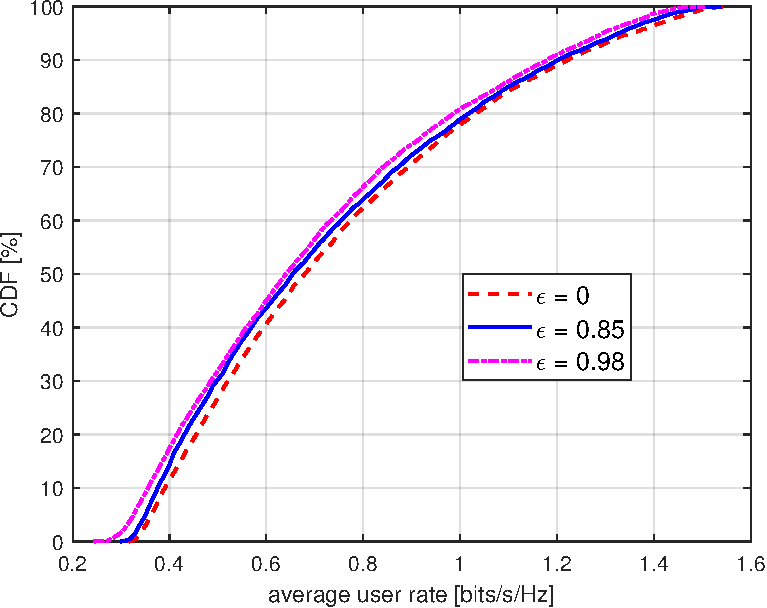
\includegraphics[width=1\linewidth]{Fig5.pdf}
    \caption{CDF of user average rate in the case of different velocity/time correlations}
    \label{fig5}
\end{figure}

\begin{figure} [htb]
    \centering
    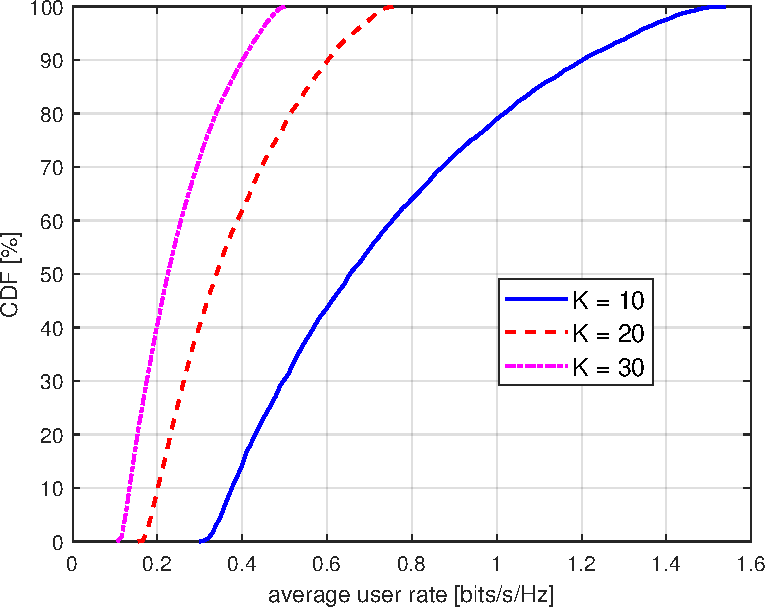
\includegraphics[width=1\linewidth]{Fig6.pdf} 
    \caption{CDF of user average rate in the case of different user numbers}
    \label{fig6}
\end{figure}

\section{Task 6: Influence of the spatial correlation}

% Figure \ref{fig7} shows the influence of the spatial correlation $t$ in \eqref{eq18}.
% According to the simulation results, if $n_r=1$, the system performance becomes better
% with the increase of $t$. However, there is an opposite situation if $n_r=2$, where the 
% performance decrease with the increase of $t$.

Figure \ref{fig7} shows the influence of the spatial correlation $t$ when $n_r=2$.
One can visualize that when $t$ approach one, there is significant decrease of the 
maximum average user rate, while a slight increase of minimum average user rate.
The explanation is given below.

\begin{figure} [htb]
    \centering
    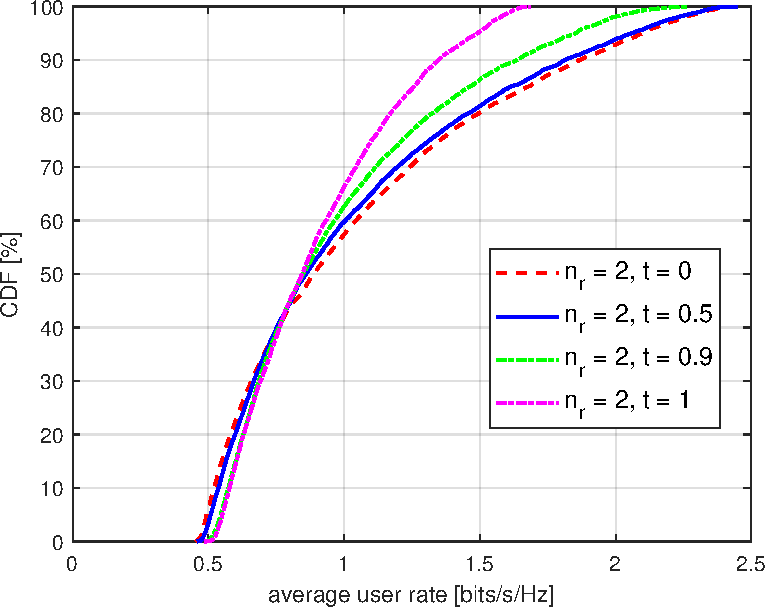
\includegraphics[width=1\linewidth]{Fig7.pdf}
    \caption{CDF of user average rate in the case of different spatial correlations for $n_r=2$}
    \label{fig7}
\end{figure}

% \subsection{$n_r=1$}
% In the case of $n_r=1$, the channel is a MISO channel and only one stream can be supported.
% Therefore, there is no inter-stream interference and the covariance matrix in \eqref{eq8} 
% becomes a scalar, which can be rewritten as $R_{\tilde{n}_q}$. The output SINR \eqref{eq11} of the MMSE receiver
% can be rewritten as 
% \begin{align}
%     \rho_q & = \frac{\Lambda_{q,i}^{-1} \left|{\bf{p}}_{q,i}^H {\bf{h}}_{q,i} \right|^2}{R_{\tilde{n}_q}} \nonumber\\
%     & = \frac{\Lambda_{q,i}^{-1} \left|{\bf{p}}_{q,i}^H ({\bf{R}}_{t,q,i}^{1/2})^H \tilde{{\bf{h}}}_{q,i} \right|^2}{R_{\tilde{n}_q}}\label{eq22}
% \end{align}
% and the achievable rate is $R_q = \log(1+\rho_q)$.

% We can rewrite the MISO channel as 
% \begin{equation}
%     {\bf{h}}_{q,i} = \left[h_{q,i,1}, h_{q,i,2}, h_{q,i,3}, h_{q,i,4}\right]^T \label{eq23}
% \end{equation}
% For the very high spatial correlation $t$, there is a linear relationship among each
% entry of the vector ${\bf{h}}_{q,i}$, i.e., if the magnitude of one entry 
% $h_{q,i,m}$ increases, the magnitudes of the others will also increase. 
% If user $q$ is scheduled, we must have all the entries of the channel vector have
% relative large at the same time because of the linear relationship. It will lead to 
% higher SINR and achievable rate. Therefore, the performance of the system is better for 
% higher $t$ when $n_r=1$.

% \subsection{$n_r=2$}

In the case of $n_r=2$, the channel is a $2 \times 4$ MIMO channel and the channel
matrix has 2 singular values, which mean there are 2 data streams can be spatially 
multiplexed in the transmission.

With the increase of the spatial correlation, the rank of the channel matrix approach 
1. For the very large spatial correlation $t$ (i.e., $t \to 1$), one of the two singular values
is almost zero. We consider the singular value decomposition (SVD) of the $2 \times 4$
channel ${\bf{H}}_{q,i}$.
\begin{align}
    {\bf{H}}_{q,i} & = {\bf{U}} \left[\begin{matrix} \sigma_{max}&0&0&0 \\ 0&\sigma_{min}&0&0 \end{matrix}\right] {\bf{V}}^H \nonumber \\
    & = {\bf{U}} \left[\begin{matrix} \sigma_{max}&0 \\ 0&\sigma_{min} \end{matrix}\right] \tilde{{\bf{V}}}^H
\end{align}
where $\tilde{{\bf{V}}}^H = {\bf{V}}^H(1:2,:)$. Therefore, the observation at \eqref{eq2} can be rewritten as
\begin{equation}
    {\bf{y}}_{q} = \Lambda_{q,i}^{-1/2} {\bf{U}} \left[\begin{matrix} \sigma_{max}&0 \\ 0&\sigma_{min} \end{matrix}\right] \tilde{{\bf{V}}}^H {\bf{x}}_{q,i} + \tilde{{\bf{n}}}_{q} 
\end{equation}
If we regard $\tilde{{\bf{V}}}^H$ as part of the transmitter and ${\bf{U}}$ as part of the 
receiver, this $2 \times 4$ MIMO channel is converted to 2 virtual SISO channels, the channel gains
of which are $\sigma_1^2$ and $\sigma_2^2$, respectively, i,e.,
\begin{equation}
    \tilde{{\bf{y}}}_q = \Lambda_{q,i}^{-1/2} \left[\begin{matrix} \sigma_{max}&0 \\ 0&\sigma_{min} \end{matrix}\right] \tilde{{\bf{x}}}_{q,i} + \tilde{{\bf{n}}}_{q} 
\end{equation}
where ${\bf{y}}_q = {\bf{U}} \tilde{{\bf{y}}}_q$ and $\tilde{{\bf{x}}}_{q,i} = \tilde{\bf{V}}^H {\bf{x}}_{q,i}$.
Therefore, there are 2 virtual streams transmitted through the channel no matter the actual 
stream is 1 or 2. As what is aforementioned, $\sigma_{min} \to 0$ as 
$t \to 1$. In this case, the channel gain of one of the virtual SISO channel would be very small, and the noise would be always 
dominant in this virtual SISO channel. 

For high SINR and low spatial correlation, $\sigma_{min}$ is 
not close to zero, and the uniform power allocation approaches the water-filling solution, which 
is capacity-achieving power allocation scheme. For the high SINR and high spatial correlation, $\sigma_{min}$
is almost zero, therefore the virtual SISO channel related to $\sigma_{min}$ cannot transmit any information.
So the maximum average user rate gets smaller when spatial correlation $t$ is larger.

For the low SINR, the channel capacity is mainly determined by $\sigma_{max}$. By keeping 
the channel gain same, the channel with higher spatial correlation will have larger $\sigma_{max}$.
Therefore, the channel with higher spatial correlation will have larger channel capacity at low SINR.
This is why the minimum average user rate of higher spatial correlation $t$ is slightly larger than 
that of lower $t$. (One related example is the Task 1 in Coursework 2).


% This interpretation in perspective of 
% singular value also explains why the performance only reduces a little from $t=0$ to $t=0.5$.
% The reason is that for the relative small value of $t$, the $\sigma_{min}$ is not very close to zero,
% and it is still large enough to recover the information under the noise.




\section{Bonus Task 1: 5G Multi-User Massive MIMO with ZFBF}
\subsection{System Model}

In this section, we consider the multi-user MIMO BC system with ZFBF.
We assume that there are total number of $K$ ($\mathcal{K} = \{1,...,K\}$) 
user equipped with single antenna and randomly distributed in the center 
cell. At each time instance $k$, the scheduled user set is denoted as ${\bf{K}} \subset \mathcal{K}$.
The transmit signal at the BS $i$ is given as
\begin{equation}
    {\bf{x}}_i = \sum_{q \in \bf{K}} {\bf{w}}_{q,i} s_q^{1/2} c_{q,i} = {\bf{W}}_i {\bf{S}}^{1/2}_i {\bf{c}}_i \label{eq22}
\end{equation}
where ${\bf{w}}_q \in \mathbb{C}^{n_t \times 1}$ is the linear precoder, which
will be designed later. $s_q$ and $c_q$ are the power allocate coefficients and 
information symbols, respectively. ${\bf{W}} = \left[{\bf{w}}_{p,i},...{\bf{w}}_{q,i}\right]_{p,q \in {\bf{K}}}$,
${\bf{S}}=\text{diag} \left\{ s_{p,i},...,s_{q,i} \right\}_{p,q \in {\bf{K}}}$, and
${\bf{c}} = \left[ c_{p,i},...,c_{q,i} \right]^T_{p,q \in {\bf{K}}}$.

The observations at all the users are
\begin{equation}
    {\bf{y}} = {\bf{H}}_i {\bf{x}}_i + \tilde{\bf{n}} = {\bf{H}}_i {\bf{W}}_i {\bf{S}}_i^{1/2} {\bf{c}}_i + \tilde{\bf{n}}\label{eq23}
\end{equation}
where
\begin{gather}
    {\bf{y}} = \left[ y_p,...,y_q \right]^T_{p,q \in {\bf{K}}} \label{eq24}\\
    {\bf{H}}_i = \left[ \Lambda_{p,i}^{-1/2} {\bf{h}}^H_{p,i},...\Lambda_{q,i}^{-1/2} {\bf{h}}^H_{q,i} \right]^T_{p,q \in {\bf{K}}} \label{eq25}\\
    \tilde{{\bf{n}}} = \sum_{j \neq i} {\bf{H}}_j {\bf{x}}_j + {\bf{n}} \label{eq26}
\end{gather}

The denormalized zero forcing precoder is given as the right pseudo inverse of ${\bf{H}}$
\begin{equation}
    {\bf{F}} = {\bf{H}}_i^H ({\bf{H}}_i {\bf{H}}_i^H)^{-1} \label{eq27}
\end{equation}
The normalized precoder ${\bf{w}}_{q,i}$ for user $q \in {\bf{K}}$ is given as
\begin{equation}
    {\bf{w}}_{q,i} = \frac{{\bf{F}}(:,q)}{ \left\Vert {\bf{F}}(:,q) \right\Vert} \label{eq28}
\end{equation}
After applying the zero forcing precoder, the intra-cell interference is eliminated at the 
user. Therefore, the observation at user $q$ is given as
\begin{align}
    y_q = &\Lambda_{q,i}^{-1/2} {\bf{h}}^H_{q,i} {\bf{w}}_{q,i} s_{q,i}^{1/2} c_{q,i} \nonumber\\
    &+ \underbrace{\sum_{j \neq i} \Lambda_{q,j}^{-1/2} {\bf{h}}^H_{q,j} {\bf{W}}_j {\bf{S}}_j^{1/2} {\bf{c}}_j}_{\text{inter-cell interference}} + n_q \label{eq29}
\end{align}

In this case, the MMSE equalizer at user $q$ is 
\begin{equation}
    g_q^{\text{MMSE}} = \Lambda_{q,i}^{-1/2} s_{q,i}^{1/2} ({\bf{h}}_{q,i}^H {\bf{w}}_{q,i})^H (R_{\tilde{n}_q})^{-1} \label{eq30}
\end{equation}
where $R_{\tilde{n}_q}$ is the covariance of the noise plus interference, and it is given as
\begin{equation}
    R_{\tilde{n}_q} = \sum_{j \neq i} \Lambda_{q,j}^{-1} {\bf{h}}_{q,j}^H {\bf{W}}_j {\bf{S}} {\bf{W}}_j^H {\bf{h}}_{q,j} + \sigma_{n_q}^2 \label{eq31}
\end{equation}

The output SINR of MMSE equalizer is 
\begin{equation}
    \rho_q = \frac{\Lambda_{q,i}^{-1} s_{q,i} \left|{\bf{h}}_{q,i}^H {\bf{w}}_{q,i} \right|^2}{R_{\tilde{n}_q}} \label{eq32}
\end{equation}
and the achievable rate is 
\begin{equation}
    R_q = \log(1+\rho_q) \label{eq33}
\end{equation}

\subsection{Proportional Fair Scheduling for Multi-user}
We denote the size of scheduled user set by $\left| {\bf{K}} \right|$. 
In order to make the zero forcing beamforming achievable, there should be 
$\left| {\bf{K}} \right| \leq n_t$. There altogether $C_K^{\left| {\bf{K}} \right|}$
possible $\left| {\bf{K}} \right|$-subsets of $\mathcal{K}$. Let $\Omega_{\left| {\bf{K}} \right|}$
denote the collection of all the possible $\left| {\bf{K}} \right|$-subsets. At each
time instance $k$, the BS will select one subset from $\Omega_{\left| {\bf{K}} \right|}$.
The optimal subset is given as 
\begin{equation}
    {\bf{K}}^* = \arg \max_{{\bf{K}} \in \Omega_{\left| {\bf{K}} \right|}} \sum_{q \in {\bf{K}}} \frac{R_q(k)}{\bar{R}_q(k)} \label{34}
\end{equation}
Actually, we also need to choose the best size of the subset ${\bf{K}}$, but in order to simplify 
the experiment and the reduce the computational cost, the $|{\bf{K}}|$ is fixed in this task.

\subsection{Numerical Results}
The parameters in Table \ref{table1} are also used in this simulation, but we assusm
that there is no spatial correlation. The size of the subset is set to $\left| {\bf{K}} \right|=4$.

\begin{figure} [htb]
    \centering
    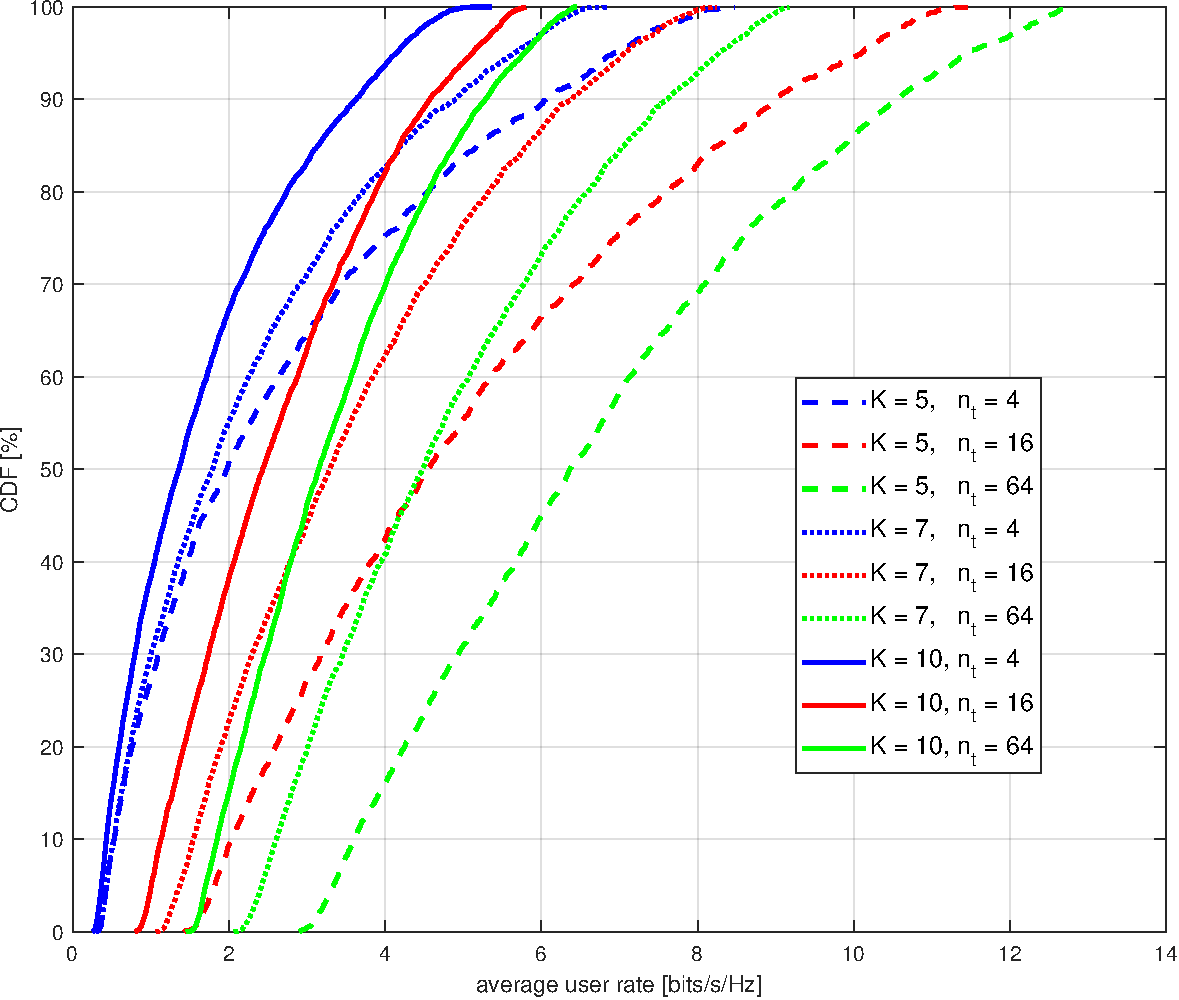
\includegraphics[width=1\linewidth]{Fig10.pdf}
    \caption{CDF of user average rate in the cases of different number of transmit antennas and users}
    \label{fig7.5}
\end{figure}

Figure \ref{fig7.5} shows the CDF of user average rate in the cases of different number of 
transmit antennas and users. It is obvious that the performance is degraded with the increase of the 
user number $K$, which is the same as the results shown in Figure \ref{fig6}.
Besides, the larger number of transmit antennas can lead to the better system performance. 
This is one of the reasons why we research the massive MIMO. 

In massive MIMO, the channel become mutually orthogonal as $n_t$ becomes large, i.e.,
\begin{equation}
    \lim_{n_t \to \infty} \frac{1}{n_t} {\bf{h}}_p^H {\bf{h}}_q = \begin{cases}
        1, p=q\\
        0, p \neq q
    \end{cases}
\end{equation}
In this case, the matrix ${\bf{H}}_i$ in \eqref{eq25} will become a unitary-like matrix, i.e.,
\begin{equation}
    {\bf{H}}_i {\bf{H}}_i^H = \text{diag}\left\{ n_t \Lambda_{p,i}^{-1},...,n_t \Lambda_{q,i}^{-1} \right\}_{p, q \in \bf{K}}
\end{equation}
and the matrix $\bf{F}$ in \eqref{eq27} becomes
\begin{equation}
    {\bf{F}} = \left[ n_t^{-1} \Lambda_{p,i}^{1/2} {\bf{h}}_{p,i},...,n_t^{-1} \Lambda_{q,i}^{1/2} {\bf{h}}_{q,i} \right]
\end{equation}
Therefore, the zero forcing precoder for user $q$ in $\bf{K}$ is 
\begin{equation}
    {\bf{w}}_{q,i} = \frac{{\bf{h}}_{q,i}}{\left\Vert {\bf{h}}_{q,i} \right\Vert}
\end{equation}
where the zero forcing beamforming becomes the matched beamforming.The zero 
forcing percoder ${\bf{w}}_{q,i}$ is parallel with the channel 
vector ${\bf{h}}_{q,i}$, due to which the value of $\left| {\bf{h}}_{q,i}^H {\bf{w}}_{q,i} \right|^2$ 
is maximized. Therefore, the user q has the maximized SINR $\rho_q$ and achievable rate $R_q$.
So as there are more transmit antennas, the channel vector gradually orthogonal to each other,
resulting in the better system performance.


\section{Bonus Task 2: Sum-rate performance of MISO NOMA and MULP}

\subsection{Multi-User MISO NOMA System}

\begin{figure} [htb]
    \centering
    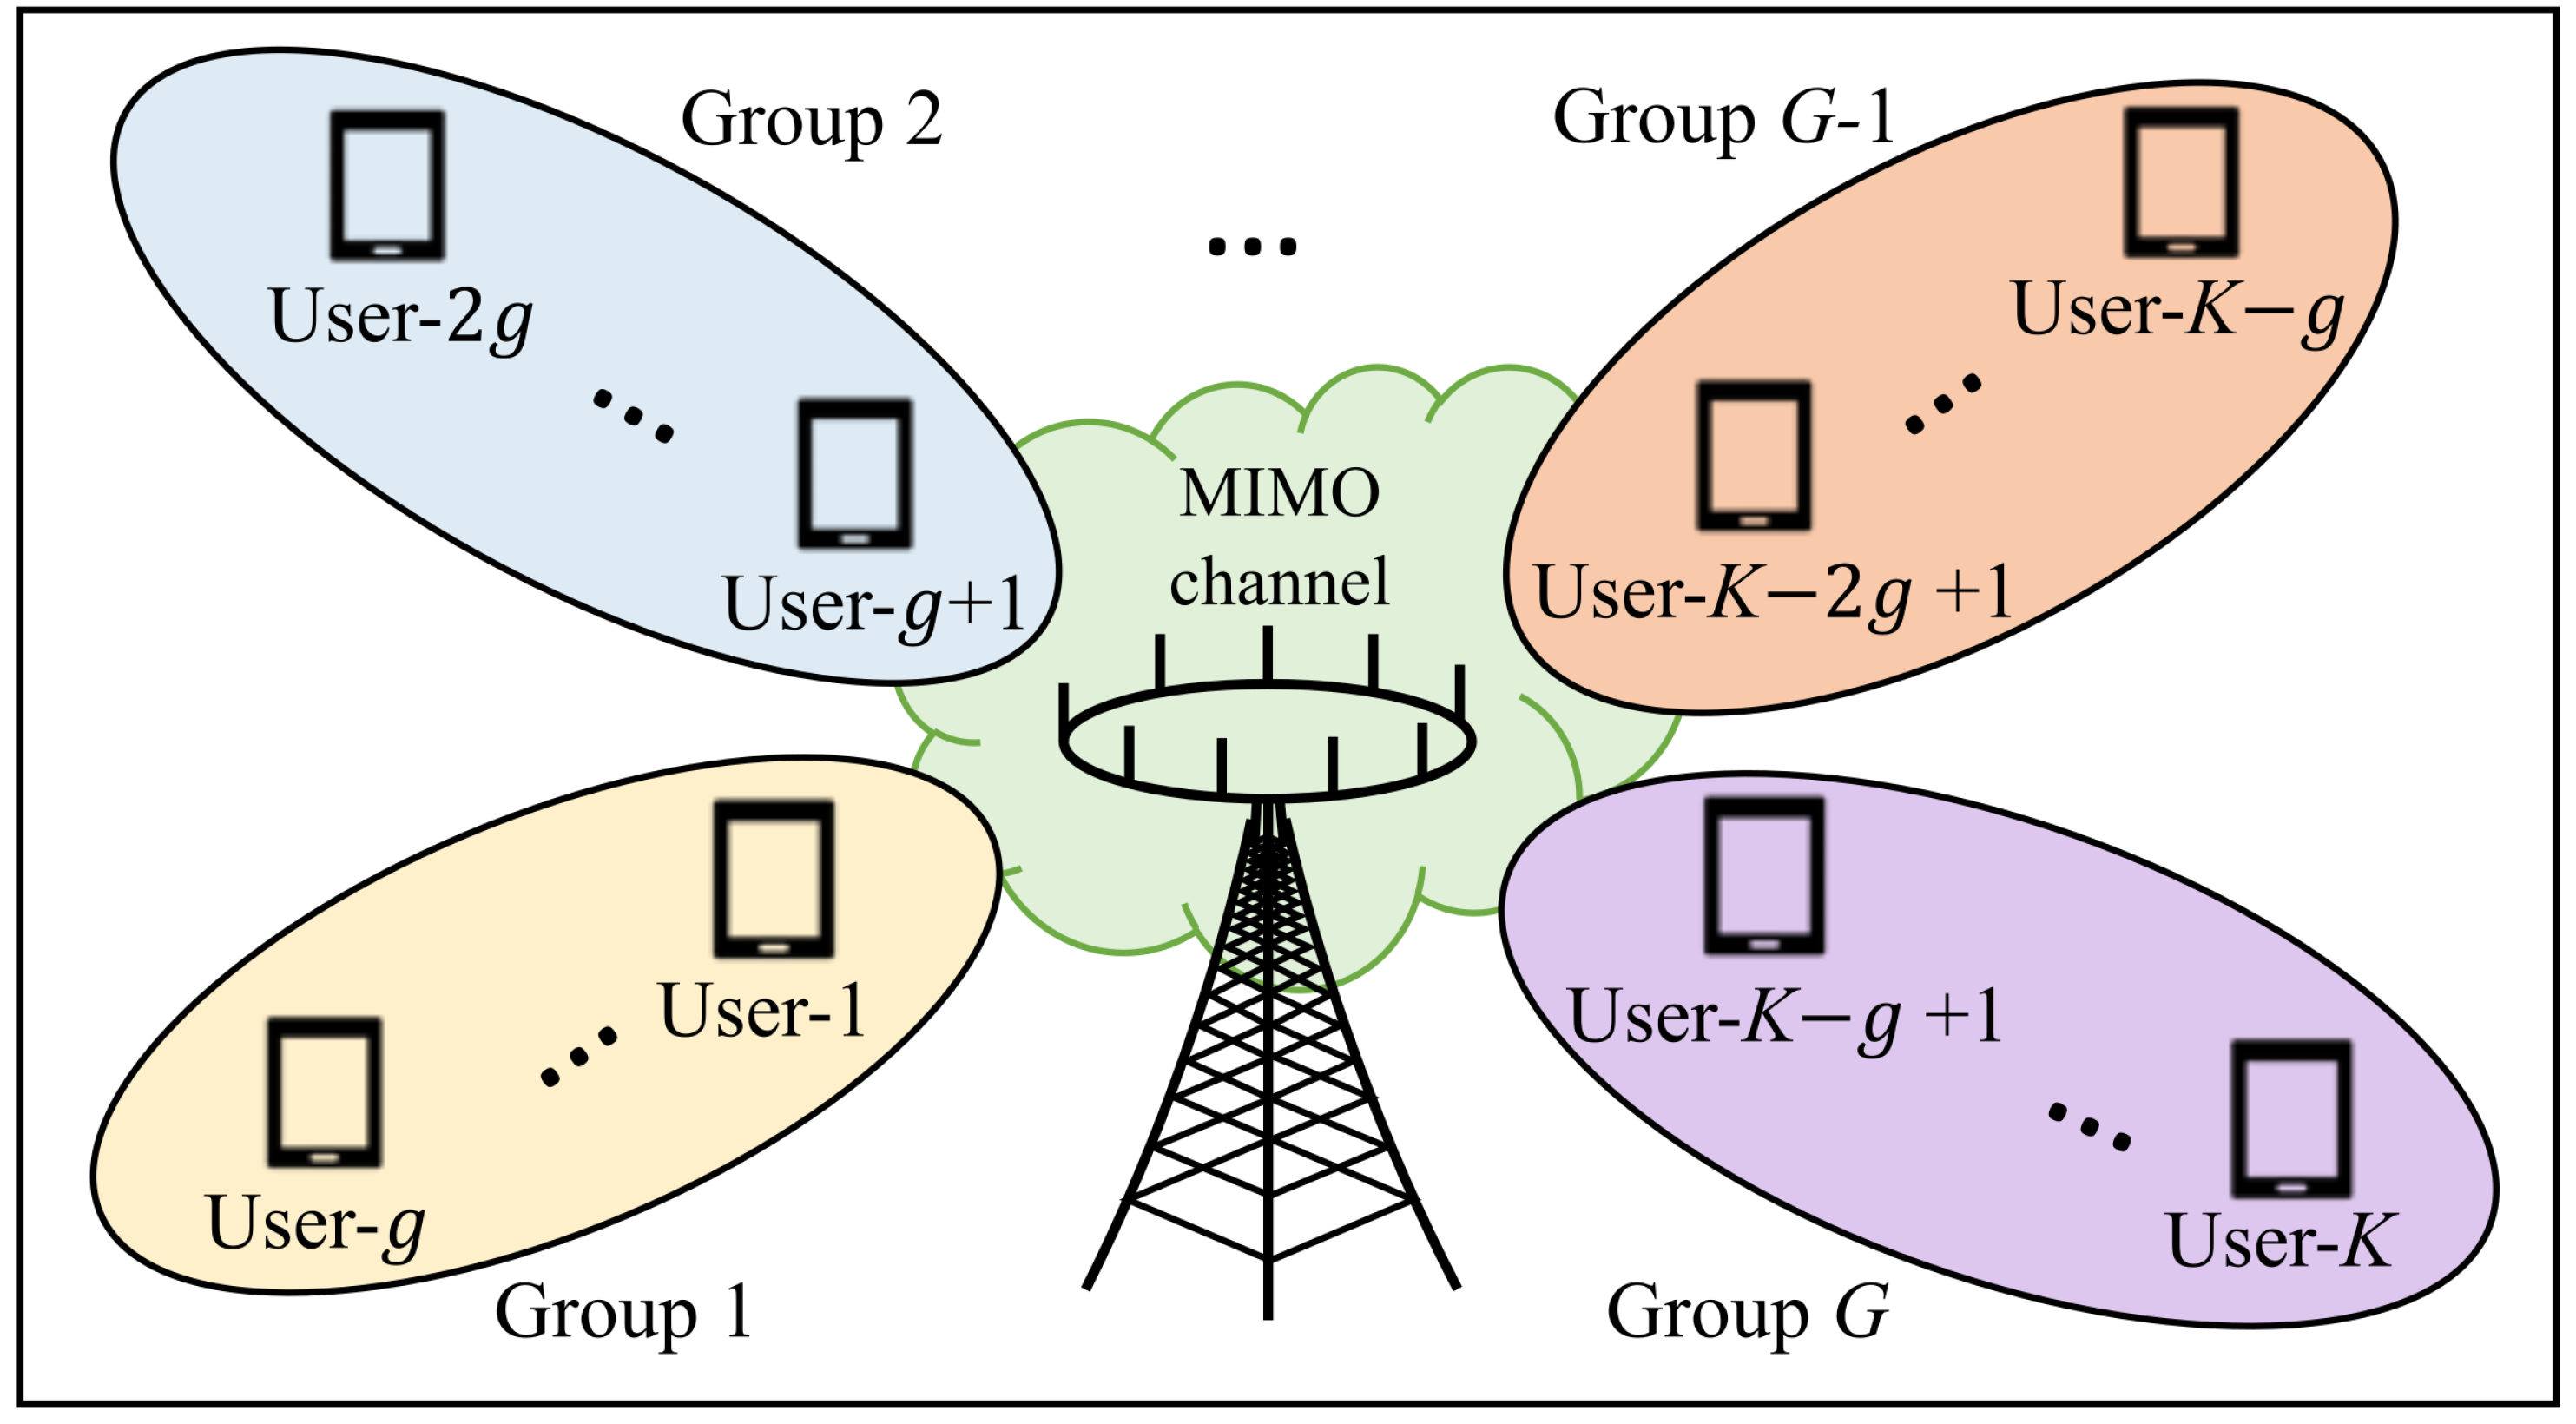
\includegraphics[width=1\linewidth]{Fig8.png}
    \caption{System architecture with MISO NOMA}
    \label{fig8}
\end{figure}

Figure \ref{fig8} shows the $K$-user MISO NOMA system. The BS is equipped with 
$M$ antenna and serving $K$ single-antenna users indexed by $\mathcal{K} = \{1,...,K\}$.
We assume that $K=gG$ which is grouped in to $G$ groups indexed by $\mathcal{G}=\{1,...,G\}$. 
The users in the $i$-th group are indexed by $\mathcal{K}_i = \{ig-g+1,...,ig\}$.

The transmit signal is given as
\begin{equation}
    {\bf{x}} = \sum_{k \in \mathcal{K}} {\bf{p}}_k s_k \label{eq37}
\end{equation}
where ${\bf{p}} \in \mathbb{C}^{M \times 1}$ is the precoder and $s_k$ is the encoded 
message for user $k$.
The signal receiver at user $k$ is 
\begin{equation}
    y_k = {\bf{h}}_k^H {\bf{x}} + n_k \label{eq38}
\end{equation}
where ${\bf{h}}_k \in \mathbb{C}^{M \times 1}$ is the channel vector and 
$n_k \sim \mathcal{CN}(0,1)$ is the complex Gaussian noise.

In group $\mathcal{K}_i$, we assume the first user is the strongest user which need to decode
the messages of the rest $g-1$ users in this group, the second one is the second strongest
user and so on. Therefore, for the user-$j \in \mathcal{K}_i$, it needs to decode the 
message of user-$\{ k | k>j, k \in \mathcal{K}_i \}$. The SINR for user-$j$ to decode
the message of user-$k$ is given as
\begin{equation}
    \rho_{j,k} = \frac{ \left| {\bf{h}}_j^H {\bf{p}}_k \right|^2 }{\underbrace{\sum_{m<k, m \in \mathcal{K}_i} \left| {\bf{h}}_j^H {\bf{p}}_m \right|^2}_{\text{intra-group interference}} + \underbrace{\sum_{l \neq i, l \in \mathcal{G}} \sum_{m \in \mathcal{K}_l} \left| {\bf{h}}_j^H {\bf{p}}_k \right|^2}_{\text{inter-group interference}} + 1}
    \label{eq39}
\end{equation}
The related rate is 
\begin{equation}
    R_{j,k} = \log_2(1 + \rho_{j,k}) \label{eq40}
\end{equation}
For user-$k$, in order to make its message decodable at each user which need to decode its messgae, 
its achievable rate is given as 
\begin{equation}
    R_k = \min_{j \leq k, j \in \mathcal{K}_i} R_{j,k} \label{eq41}
\end{equation}

If there is no inter-group interference, the $R_{j,k}$ is upper bounded by
\begin{equation}
    R_{j,k} \leq \log_2 \left( 1 + \frac{ \left| {\bf{h}}_j^H {\bf{p}}_k \right|^2 }{1 + \sum_{m<k, m \in \mathcal{K}_i} \left| {\bf{h}}_j^H {\bf{p}}_m \right|^2} \right) \label{eq42}
\end{equation}
For $R_k$, if $R_{ig-g+1,k}$ (the first one in $\mathcal{K}_i$) is the minimum one for all $j \leq k, j \in \mathcal{K}_i$, we have
$R_k = R_{ig-g+1,k}$. Otherwise, we have $R_k < R_{ig-g+1,k}$. Therefore, $R_k$ is upper bounded by
\begin{align}
    R_k &\leq R_{ig-g+1,k} \nonumber \\
    &\leq \log_2 \left( 1 + \frac{ \left| {\bf{h}}_{ig-g+1}^H {\bf{p}}_k \right|^2 }{1 + \sum_{m=ig-g+1}^{k} \left| {\bf{h}}_{ig-g+1}^H {\bf{p}}_m \right|^2} \right)\label{eq43}
\end{align}
The sum rate for group $\mathcal{K}_i$ is upper bounded by
\begin{align}
    &\sum_{k=ig-g+1}^{ig} R_k \nonumber \\
    &\leq \sum_{k=ig-g+1}^{ig} \log_2 \left( 1 + \frac{ \left| {\bf{h}}_{ig-g+1}^H {\bf{p}}_k \right|^2 }{1 + \sum_{m=ig-g+1}^{k} \left| {\bf{h}}_{ig-g+1}^H {\bf{p}}_m \right|^2} \right) \nonumber \\
    & = \log_2 \left( 1 + \sum_{k=ig-g+1}^{ig} \left| {\bf{h}}_{ig-g+1}^H {\bf{p}}_k \right|^2 \right)
\end{align}

The $R_k$ can be further upper bounded using Cauchy-Schawarz ineuqality.
\begin{align}
    \sum_{k=ig-g+1}^{ig} R_k &\leq \log_2 \left( 1 + \sum_{k=ig-g+1}^{ig} \left| {\bf{h}}_{ig-g+1}^H {\bf{p}}_k \right|^2 \right) \nonumber \\
    & \leq \log_2 \left( 1 + \left\Vert{\bf{h}}_{ig-g+1}\right\Vert ^2 \sum_{k=ig-g+1}^{ig} \left\Vert {\bf{p}}_k \right\Vert^2 \right) \nonumber \\
    & = \log_2 \left( 1 + \left\Vert{\bf{h}}_{ig-g+1}\right\Vert ^2 w_i P \right)
\end{align}
where $w_i P$ is the power allocated to the group $\mathcal{K}_i$ and $P$ is the overall transmit power.
In this case, the overall sum rate is upper bounded by
\begin{equation}
    R_s = \sum_{k=1}^K R_k \leq \sum_{i=1}^G \log_2 \left( 1 + \left\Vert{\bf{h}}_{ig-g+1}\right\Vert ^2 w_i P \right) \label{46}
\end{equation}
Therefore, we can obtain the multiplexing gain of the $K$-user MISO NOMA system
\begin{equation}
    d_s \leq \lim_{P \to \infty} \frac{\sum_{i=1}^G \log_2 \left( 1 + \left\Vert{\bf{h}}_{ig-g+1}\right\Vert ^2 w_i P \right)}{\log_2 (P)} = G \label{eq47}
\end{equation} 
Additionally, for a MIMO system with $M$ transmit antennas and $K$ single-antenna users,
the maximum achievable multiplexing gain is $\min\{ M,K \}$. So we have $d_s \leq \min\{M,K,G\}$.
Since $G < K$, the multiplexing gain of the NOMA system is upper bounded by
\begin{equation}
    d_s \leq \min \{ M,G \} \label{eq47}
\end{equation}

\subsection{Multi-User Linear Precoding System}
\begin{figure} [htb]
    \centering
    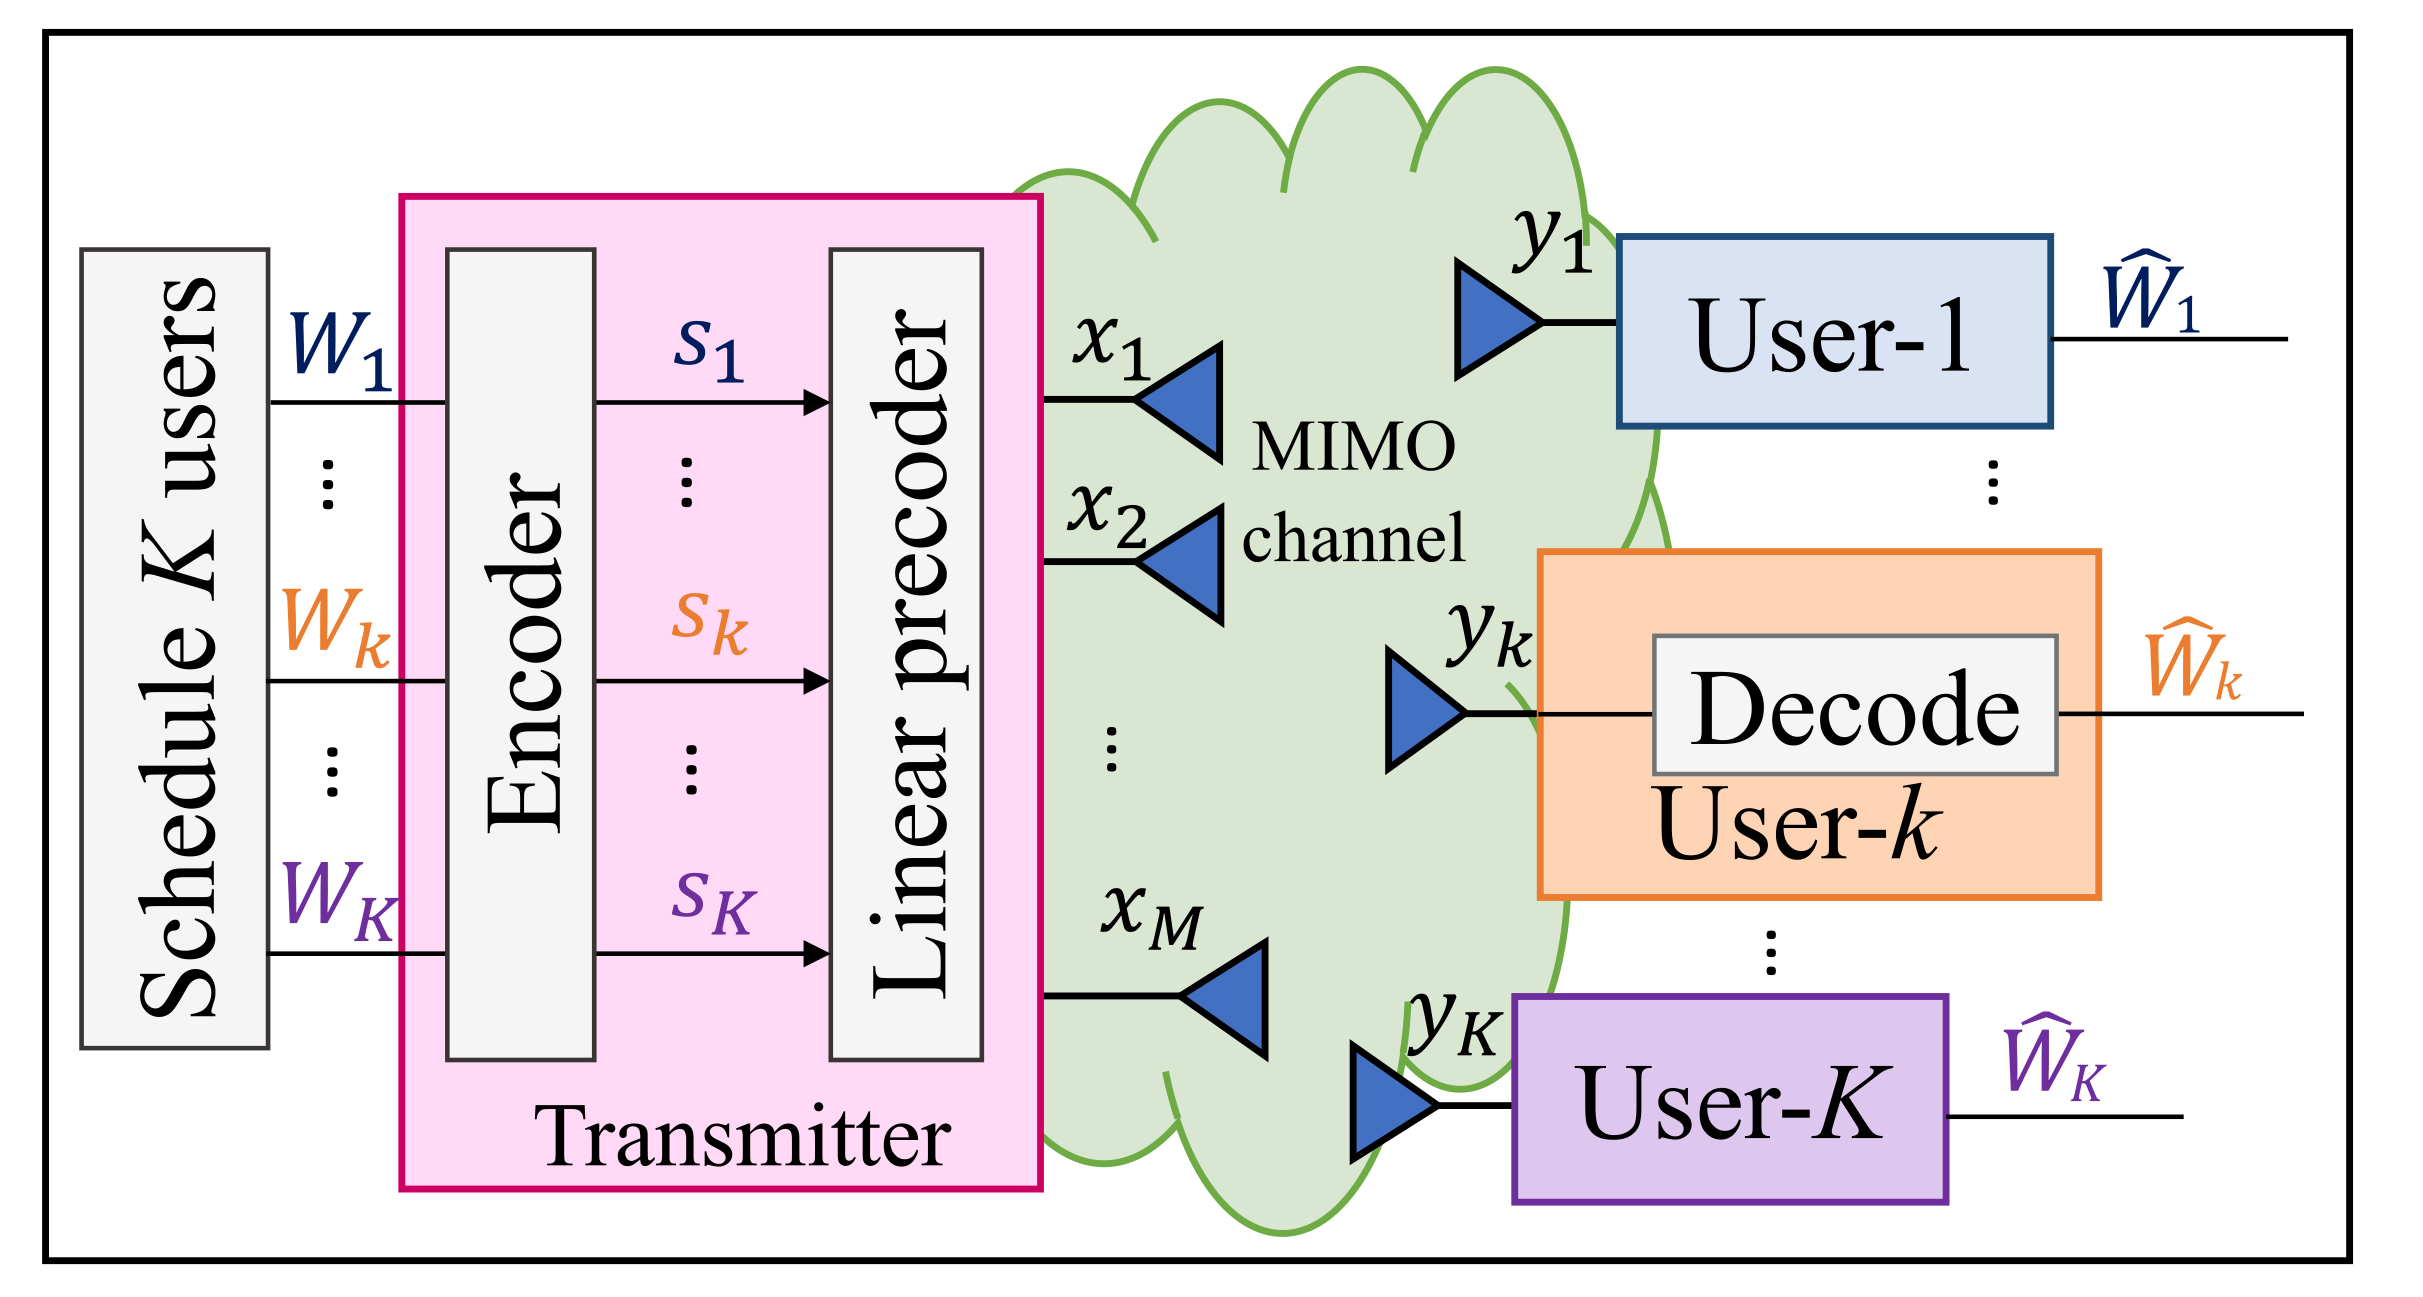
\includegraphics[width=1\linewidth]{Fig9.png}
    \caption{System architecture with MISO MULP}
    \label{fig9}
\end{figure}

Figure \ref{fig9} shows the system architecture with MISO MULP. The system has the same 
setup as the previous MISO NOMA system, but the linear precoding  instead of superposition coding
is applied at the BS. The transmit signal is given as 
\begin{equation}
    {\bf{x}} = \sum_{k \in \mathcal{K}} {\bf{p}}_k s_k \label{49}
\end{equation}
The signal received at user $k$ is
\begin{equation}
    y_k = {\bf{h}}_k^H {\bf{p}}_k s_k + \underbrace{\sum_{j \in \mathcal{K}, j \neq k} {\bf{h}}_k^H {\bf{p}}_j s_j}_{\text{interference}} + n_k \label{51}
\end{equation}
The SINR at user $k$ is
\begin{equation}
    \rho_k = \frac{\left| {\bf{h}}_k^H {\bf{p}}_k \right|^2}{\sum_{j \in \mathcal{K}, j \neq k} \left| {\bf{h}}_k^H {\bf{p}}_j \right|^2 + 1}
\end{equation}
and the achievable rate is $R_k = \log_2(1+\rho_k)$. We assume the zero forcing precoding is exploited,
then we have ${\bf{h}}_k^H {\bf{p}}_j = 0, k \neq j$. The achievable rate can be written as
\begin{align}
    R_k &= \log_2 (1 + \left| {\bf{h}}_k^H {\bf{p}}_k \right|^2) \nonumber \\
    &\leq \log_2 (1 + \left\Vert {\bf{h}}_k \right\Vert^2 \left\Vert{\bf{p}}_k \right\Vert^2) \nonumber\\
    & = \log_2 (1 + \left\Vert {\bf{h}}_k \right\Vert^2 w_k P) \label{eq51}
\end{align} 
where $w_k P$ is the power allocated to user $k$ and $P$ is the overall transmit power. Therefore,
the multiplexing gain of the MULP with ZF is 
\begin{equation}
    d_s \leq \lim_{P \to \infty} \frac{\sum_{k=1}^K \log_2 (1 + \left\Vert {\bf{h}}_k \right\Vert^2 w_k P)}{\log_2(P)} = K \label{53}
\end{equation}
However, the ZF precoding can support all the $K$ users only if $K \leq M$. When $M \leq K$,
the ZF precoding can only support $M$ users simultaneous and the scheduling is needed, where the multiplexing gain
is upper bounded by $M$. Therefore, we have
\begin{equation}
    d_s \leq \min\{M,K\} \label{eq54}
\end{equation}

It is obvious that the MULP outperforms the NOMA in terms of multiplexing gain.

\end{document}


